\begin{figure}[t]
    \centering
    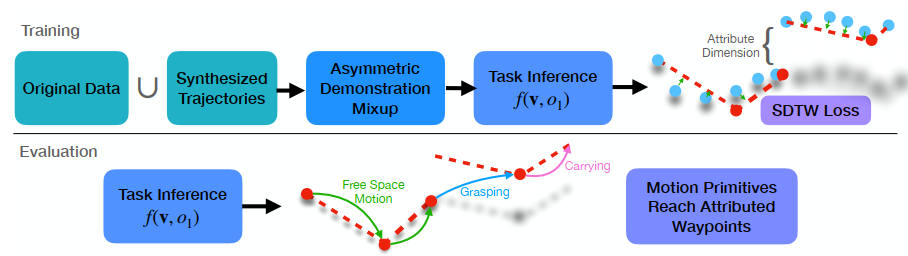
\includegraphics[width=0.9\textwidth]{figures/images/awda/awda_framework.png}
    \caption{AWDA framework proposed in \cite{chang2023one}. The task inference network $f(v,o)$ predicts a sequence of attributed waypoints (red dots) that are achieved by hand-defined motion primitives. The original data are augmented with free-space motion trajectories and asymmetric demonstration mixup in order to reduce the correlation between tasks and task content.}
    \label{fig:awda_framework}
\end{figure}
